\documentclass{article}

% Language setting
% Replace `english' with e.g. `spanish' to change the document language
%\usepackage[]{babel}

\usepackage[letterpaper,top=2cm,bottom=2cm,left=3cm,right=3cm,marginparwidth=1.75cm]{geometry}

% Useful packages
\usepackage{amsmath}
\usepackage{graphicx}
\usepackage[colorlinks=true, allcolors=blue]{hyperref}
\usepackage{hhline}
\usepackage{tabularx}
\usepackage{float}

\title{Wechselstrom-Widerstandsbestimmung}
\author{Lukas Babitschew, Phil Gith, Stefan Ertl}

\begin{document}
\maketitle


\section{Versuchsziel}

Im folgenden Versuch sollen verschiedene reale Wechselstromwiderstände gemessen werden. Jeder Widerstand wurde mit drei verschiedenen Methoden bemessen: Drei-Spannungs-Messer-, Drei-Strom-Messer-Methode und mit einem LCR Messgerät.

\section{Versuchsaufbau}

\begin{table}[H]
\centering
\begin{tabular}{|l||l|l|}
\hline
Fluke Digitalmultimeter & & \\ \hline
Fluke Digitalmultimeter & & \\ \hline
Hameg Leistungsmessgerät & & \\ \hline
\end{tabular}
\caption{Messwerte}
\end{table}


\section{Versuche}
\subsection{UIP-Messung}
\begin{figure}[H]
\centering
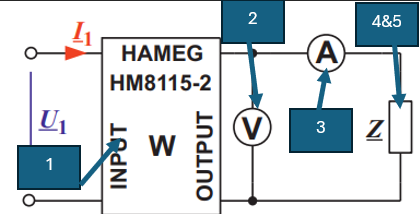
\includegraphics[width=0.75\linewidth]{leistung.png}
\caption{Schaltbild Leistungsmessung}
\end{figure}

\begin{enumerate}
	\item Hameg Leistungsmessgerät
	\item Fluke Digitalmultimeter als Spannungsmesser
	\item Fluke Digitalmultimeter als Strommesser
	\item Untersuchter Kondensator
	\item Untersuchte Spule
\end{enumerate}

Um den Betrag des Widerstandes zu berechnen, wird zunächst Strom und Spannung gemessen. Daraus lässt sich berechnen:
\[
	|Z| = \frac{U}{I}
\]
\[
	|S| = U \cdot I
\]
Mit Hilfe des Leistungsmessgerätes kann nun die Wirkleistung des Systems gemessen werden. Daraus ergibt sich der Phasenwinkel des Widerstands mit:

\[
	\phi = \arccos(\frac{P}{S})
\]

Allerding kommt es bei gleichzeitiger Strom und Spannungsmessung immer zu kleinen Ungenauigkeiten, da ein Messgerät das andere mitmisst.\\
Je nach dem welcher Wert korrekt gemessen wird ist der Aufbau entweder Strom- oder Spannungsrichtig.
Bei der UIP Messung ist die stromrichtige Schaltung sinnvoller. Bei einer spannungsrichtigen Schaltung liegt der Spannungspfad direkt am Prüfling wodurch das Amperemeter den Strom durch den Prüfling und den Eigenstrom des Spannungspfades misst. Dies wäre sinnvoll, wenn der Prüfling sehr niederohming ist. Bei der stromrichtigen Schaltung widerum liegt der Strompfad in Reihe mit dem Prüfling, weswegen das Voltmeter über beide hinweg misst. Der Spannungsabfall wird hier am Amperemeter mitgemessen. Da der Innenwiderstand des HAMEG HM815-2 sehr klein ist und die Impedanzen im Vergleich äußerst hochohmig sind, fällt am Strompfad kaum Spannung ab. Somit ist der systematische Messfehler hier deutlich geringer.

\subsection{•}



\end{document}